\chapter{Quantitative Methods to Measure Renal Oxygenation}
\label{chap:TRUST}
\newpage
\begin{abstract}
	Measurements of oxygenation of blood entering and leaving the kidneys would be a highly desirable quantitative biomarker allowing the calculation of renal metabolic rate of oxygen. Two methods of measuring blood oxygen saturation using \acs{MRI} are used in the brain,  \ac{SBO} and \ac{TRUST}.
	
	Here both methods are tailored for use in the abdomen, these modified sequences are compared to their unmodified counterparts in the controlled environment of the brain, verifying that the modifications do not alter the quantitative accuracy. The methods are then applied to measure oxygenation in the renal vein. The geometry of the renal vessels leads to a high degree of uncertainty when applying \ac{SBO}, however \ac{TRUST} produced results concordant with literature.
	
	To verify the \ac{TRUST} was able to measure a change in renal oxygenation, a hyperoxia challenge was undertaken. Measurements of oxygen saturation in the renal vein were collected using \ac{TRUST} and \acs{BOLD} \ttwostar maps, the current standard for assessing renal oxygenation, were collected while the subject was breathing room air, then pure oxygen. A 16~$\pm$~3~\% increase in oxygenation was measured using \ac{TRUST} whereas no significant difference in \ttwostar could be detected. 
	
	\textit{This work was presented as an oral presentation at the \ac{ISMRM} 26th Annual Meeting (2018) \cite{daniel_applying_2018}.}
	
%	\lipsum[1]
\end{abstract}
\newpage
\acresetall

\section{Introduction}
As part of a multiparametric quantitative \ac{MRI} protocol, Section \ref{sec:intro_clinical}, properties such as haemodynamics, oxygenation, and microstructure are assessed in a single 45 minute scanning session \cite{cox_multiparametric_2017, buchanan_quantitative_2019}. Currently renal oxygenation is typically assessed by using \ac{BOLD} \ttwostar/$R_2^*$ maps to infer oxygenation of different tissues within the kidney, predominately the separation in mean \ttwostar between the renal cortex and medulla, an example of which is shown in Figure \ref{fig:T2*map}. These \ac{BOLD} \ttwostar maps are, however, affected by other factors such as susceptibility effects, shimming and baseline blood flow and thus may be limited in their ability to draw quantitative conclusions despite their widespread use \cite{pruijm_blood_2017}. For a detailed review of these confounding factors see Niendorf \textit{et al} \cite{niendorf_how_2014}. More recently it has been suggested that the gradient in the \ttwostar/$R_2^*$ across the corticomedullary interface may provide a better biomarker of renal oxygenation \cite{milani_reduction_2017, pruijm_blood_2017}.

\begin{figure}[H]
	\centering
	\includegraphics[width=0.45\textwidth]{TRUST/T2star_map.eps}
	%\missingfigure{T2* Map}
	\caption{An example \ttwostar map. A clear difference can be seen between the renal medulla and cortex.}
	\label{fig:T2*map}	
\end{figure}

A welcome addition to this multiparametric model would be the assessment of \ac{RMRO$_2$}; a measure analogous to the \ac{CMRO$_2$} \cite{chong_cerebral_2015}. This measure can be calculated via Equation \eqref{eq:RMR02},
\begin{equation}
\textup{RMRO}_{\textup{2}} = \left( Y_a - Y_v \right) \times \textup{RBF} \times \left[\textup{Hct}\right]
\label{eq:RMR02}
\end{equation}
where $Y_a$ and $Y_v$ are arterial and venous oxygen saturation respectively, \acsu{RBF} is renal blood flow (in m$\ell$/min) and Hct is the ratio of the volume of erythrocytes to the volume of the rest of the blood, known as haematocrit. \ac{RBF} can be measured relatively easily using \ac{PC}-\ac{MRI} \cite{jordan_velocity_1994} and Hct is usually of the order of 0.41 for healthy adults but can be measured from a simple blood test \cite{miao_reference_2002, gardener_dependence_2010} or established using the correlation between the \tone of blood and its haematocrit \cite{shimada_vivo_2012}. This means that only a measurement of blood oxygen saturation in the renal vein via a non-invasive protocol is required to generate a quantitative value of \ac{RMRO$_2$}.

Blood oxygen saturation can be measured precisely via the insertion of catheters into the subject, however this is clearly an invasive process which is not viable in humans \cite{nagdyman_comparison_2005}. There are currently two well established methods of measuring blood oxygenation via \ac{MRI}, however thus far these techniques have only been used to measure oxygen saturation in the sagittal sinus, a prominent vein in the brain. These methods are \ac{TRUST} \cite{lu_quantitative_2008, xu_improving_2012, liu_testretest_2013, liu_multi-site_2016} and \ac{SBO} \cite{jain_mri_2010, jain_cerebral_2014, driver_global_2014, lee_multiplexed_2017}. \ac{TRUST} builds on the idea of \ac{ASL} in the fact that by subtracting control images from label images an image of only blood is generated. However, instead of labelling a slab of tissue in the neck and imaging a superior slice in the brain, when implementing \ac{TRUST} the imaging plane is inferior to the label slab allowing a difference image of the blood in the sagittal sinus to be generated. By collecting a series of pairs of label and control images with different \ttwo weightings it is possible to fit the data from the sagittal sinus to a \ttwo relaxation, and using a calibration curve to convert the value of \ttwo in the sagittal sinus to venous oxygenation \cite{wright_estimating_1991}. \ac{SBO} is based on the differences in magnetic susceptibility between the blood and the surrounding tissue. Using a phase map it is possible to model this difference in susceptibility and using the known difference in susceptibility between fully oxygenated blood and fully deoxygenated blood, venous oxygenation can be calculated.

Here both of the above techniques are applied to study oxygenation in the renal vein in young healthy individuals to assess the technicalities of transferring these protocols from the brain to the body. Given that these techniques have already been used in the brain with a number of studies in the literature, the sequences are first implemented on the brain to assess oxygenation in the superior sagittal sinus, then adapted to work within the more challenging environment of applications within the abdomen. These adapted sequences are compared to the results gained using the standard implementation in the brain before testing on the renal vein. Finally oxygen challenge is carried out to verify that changes in oxygenation can be measured in the renal vein. If proved successful these sequences will be incorporated into the multiparametric renal \ac{MRI} protocol.

\section{Methods}

Imaging was performed on a whole body 3 Tesla \ac{MRI} scanner (Ingenia, Philips Medical Systems, The Netherlands) using a 32 channel head or body coil. Studies were carried out according to the principles of the Declaration of Helsinki and approved by either the Local Ethics Committee or the East Midlands Research Ethics Committee. Written informed consent was obtained from all subjects.

\subsection{Susceptibility-Based Oximetry}
\label{sec:SBO}
\subsubsection{\ac{MRI} Protocol}
\label{sec:SBO_prot}
The principle behind \ac{SBO} is based on the fact that there is a difference in magnetic susceptibility between the blood within a vessel and the tissue surrounding it \cite{haacke_vivo_1997}. As outlined by Jain \textit{et al} \cite{jain_mri_2010}, if a blood vessel is modelled as a long paramagnetic cylinder, it is possible to calculate the oxygenation of the blood by knowing the phase difference between the blood in the vessel and the surrounding tissue, the angle ($\theta$) of the vessel to the static field, $B_0$, the echo time of the scan and the subject's haematocrit, Hct. This relationship is given by,
\begin{equation}
\textup{Y}_{\textup{v}} = \left[ 1-\frac{2|\Delta\phi|}{\gamma TE\Delta\chi_{\textup{do}}B_0(\cos^2\theta-1/3)\textup{Hct}}\right]\times 100,
\label{eq:SBO}
\end{equation}
where $\Delta\phi$ is the average phase difference between the blood in the vessel and the surrounding tissue, $\gamma$ is the gyromagnetic ratio of a proton, $\Delta\chi_{\textup{do}}$ is the susceptibility difference between fully deoxygenated and fully oxygenated blood ($4\pi\times0.27\textup{p.p.m}$) \cite{spees_water_2001, jain_investigating_2012}. Given the haematocrit can be assumed or measured with a blood test or by measuring the \tone of the blood \cite{lu_determining_2004}, this means that from a simple phase map it is possible to calculate $Y_v$. The optimum phase map for this purpose was produced using a 2D \tone-weighted \ac{FFE} sequence with a flip angle of $25\degree$, flow compensation, coil homogeneity correction and flyback. The \ac{FOV} was 230$\times$184$\times$29 mm, matrix size of 400$\times$300, \ac{TR} of 12 ms, \ac{TE} of 7.5 ms and three signal averages. This led to a total acquisition time of 9 seconds and as such could be completed in a single breath hold if required when moved to a body imaging protocol.

\subsubsection{Analysis}

A \ac{ROI} containing the superior sagittal sinus was defined on the phase map. This mask was then dilated with concentric shells to generate the two \ac{ROI} shown in Figure \ref{fig:SBO_ROI}, note that the outer \ac{ROI} has been constrained to within the brain during its dilation. There were no occurrences of phase wrapping in or immediately surrounding the superior sagittal sinus observed due to its small size and the high field homogeneity within the head and of the 3T scanner used. Any occurrences of phase wrapping could easily be corrected using \ac{PRELUDE}, a tool within \ac{FSL} (fMRIB, The University of Oxford) \cite{jenkinson_fast_2003}. The average values of phase within these two \acp{ROI} along with the angle of the vessel to the $B_0$ field, $\theta$, as calculated from the localisation scans and used together with Equation \eqref{eq:SBO} to calculate $Y_v$.

\begin{figure}[H]
	\centering
	\includegraphics[width=0.6\textwidth]{TRUST/SBO_ROI}
	\caption{The region of interest averaged to find the intra-vascular phase (blue) and the region of interest used to find the phase of the surrounding tissue (red).}
	\label{fig:SBO_ROI}	
\end{figure}


\subsection{\ttwo Relaxation Under Spin Tagging}

\subsubsection{\ac{MRI} Protocol}
\label{sec:TRUST_MRI}

The protocol for the \ac{TRUST} \ac{MRI} sequence in the brain involves the acquisition of a series of paired images using the pulse sequence shown in Figure \ref{fig:TRUST_TILT_Seq}. A series of four presaturation pulses using the \ac{WET} scheme ($\theta_1 = 88.9\degree$, $\theta_2 = 98.7\degree$, $\theta_3 = 82.5\degree$, $\theta_4 = 159\degree$) are applied to the imaging slice, shown in Figure \ref{fig:TRUST_Brain}, to reduce the signal from static tissue and reduce contamination of the magnetisation in the imaging slice by an imperfect labelling slab profile \cite{hendrikse_measurements_2003}. This choice of flip angles for the \ac{WET} scheme has been shown to be very efficient at providing saturation over a wide range of \tone values \cite{golay_pulsed_2005}. In the first of each image pair, a label scheme is applied consisting of two successive slice-selective $90\degree$ \ac{RF} pulses to generate a $180\degree$ label. The next image in the sequence is following a control scheme instead of the labelling scheme; for this the second of the $90\degree$ pulses is applied $180\degree$ out of phase to result in zero net effect. As such any effects of magnetisation transfer related signal in the stationary tissue can be cancelled out because the net \ac{RF} effect on the macromolecular spin magnetization is identical for both the labelling pulse and control pulse. This method of labelling is known as \ac{TILT} and is widely used in literature for \ac{TRUST} in the brain \cite{golay_transfer_1999}. A series of non-selective \ttwo preparation pulses are then applied to minimise the blood outflow effect and modulate the \ttwo weighting of the image as in the \ac{CPMG} sequence described in Chapter \ref{chap:t2_mapping}, the time between the application of the labelling pulse and the \ttwo preparation is known as the \ac{PLD}. Finally a $90\degree$ excitation pulse is applied followed by a standard \ac{EPI} readout at time \ac{TE} later \cite{xu_improving_2012}. If the control image is subtracted from the label image then only the venous blood that flowed from the label slab to the imaging slice will be visible, as shown in Figure \ref{fig:SS_labsub}.

\begin{figure}[H]
	\centering
	\begin{subfigure}[c]{1.0\textwidth}
		\centering
		\includegraphics[width=1\textwidth]{TRUST/TRUST_TILT.eps}
		\caption{}
		\label{fig:TRUST_TILT_Seq}
	\end{subfigure}
	\vskip\baselineskip
	\begin{subfigure}[c]{0.8\textwidth}
		\centering
		%\missingfigure{TRUST_TILT_Brain.ai from ISMRM presentation}
		\includegraphics[width=0.6\textwidth]{TRUST/TRUST_TILT_Brain.eps}
		\caption{}
		\label{fig:TRUST_Brain}
	\end{subfigure}
	\caption{(\subref{fig:TRUST_TILT_Seq}) The pulse sequence for \ac{TRUST} \ac{MRI} which is implemented using the standard TILT labelling scheme. (\subref{fig:TRUST_Brain}) The labelling and imaging volumes used for TILT within the brain, note that the labelling is applied above the sagittal sinus.}
	\label{fig:TRUST_TILT}
\end{figure}

\begin{figure}[H]
	\centering
	\begin{subfigure}[c]{0.30\textwidth}
		\centering
		\includegraphics[width=1\textwidth]{TRUST/Brain_Control}
		\caption{}
		\label{fig:SS_cont}
	\end{subfigure}
	\hfill
	\begin{subfigure}[c]{0.30\textwidth}
		\centering
		\includegraphics[width=1\textwidth]{TRUST/Brain_Label}
		\caption{}
		\label{fig:SS_lab}
	\end{subfigure}
	\hfill
	\begin{subfigure}[c]{0.30\textwidth}
		\centering
		\includegraphics[width=1\textwidth]{TRUST/Brain_eTE_1}
		\caption{}
		\label{fig:SS_diff}
	\end{subfigure}
	\caption{The \ac{TILT} control image (\subref{fig:SS_cont}) is subtracted from the label image (\subref{fig:SS_lab}) to generate  a difference image (\subref{fig:SS_diff}) of only the labelled venous blood in the sagittal sinus.}
	\label{fig:SS_labsub}
\end{figure}

This process is then repeated for another pair of images, with the duration of the \ttwo preparation increased to a larger \ac{eTE}, which applies a \ttwo weighting to the image in addition to the constant weighting caused by the regular \ac{TE}. Three label/control image pairs were acquired at each \ac{eTE} of 1 ms, 40 ms, 80 ms and 160 ms.

The resulting signal in the superior sagittal sinus of the difference between the label and control image, $\Delta S$, is defined by Equation \eqref{eq:TRUST}
\begin{alignat}{2}
	S_{\text{label}} &=\left(1-2\cdot e^{\sfrac{-\left(TI - eTE\right)}{\tone}}\right) \cdot & &e^{\sfrac{-eTE}{\ttwo}} \cdot e^{\sfrac{-TE}{\ttwostar}} \\
	S_{\text{control}} &= & &e^{\sfrac{-eTE}{\ttwo}} \cdot e^{\sfrac{-TE}{\ttwostar}} 
\end{alignat}  
\begin{alignat}{1}
	\Delta S&=S_{\text{label}}-S_{\text{control}}\nonumber\\
	&= 2\cdot e^{\sfrac{-\left(TI - eTE\right)}{\tone}} \cdot e^{\sfrac{-eTE}{\ttwo}} \cdot e^{\sfrac{-TE}{\ttwostar}} \nonumber\\
	&= 2 \cdot e^{-\sfrac{TI}{T_1}-\sfrac{TE}{T_2^*}} \cdot e^{eTE\left(\sfrac{1}{T_1}-\sfrac{1}{T_2}\right)}\nonumber\\
	&=S_0 \cdot e^{eTE\left(\sfrac{1}{T_1}-\sfrac{1}{T_2}\right)}
	\label{eq:TRUST}
\end{alignat}  
where $S_0=2 \cdot e^{-\sfrac{TI}{T_1}-\sfrac{TE}{T_2^*}}$ and; \tone, \ttwo and \ttwostar are the relaxation constants of blood \cite{lu_quantitative_2008}. If it is assumed that \tone of blood is approximately 1624 ms at 3T \cite{lu_determining_2004} then it is possible to fit the collected data to a mono-exponential function and estimate of \ttwo. It is deemed acceptable to use a mean value of \tone as it will always be much greater than the value of \ttwo and thus the possible small changes in blood \tone due to the oxygenation level and haematocrit become negligible when fitting the \ttwo curve.

The final step in this procedure is to convert the value of \ttwo into one of venous oxygenation, $Y_v$. The relationship between \ttwo and $Y_v$ is well studied and a simple empirically derived calibration curve can be used for this conversion, Figure \ref{fig:calibration_curve} \cite{gardener_dependence_2010, silvennoinen_comparison_2003, liu_t1_2016}.

\begin{figure}[H]
	\centering
	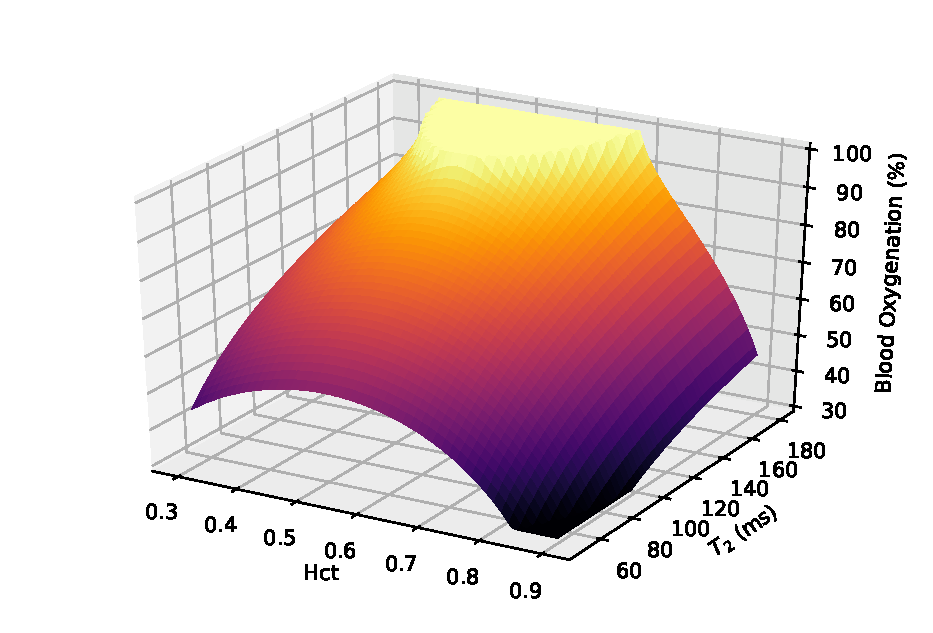
\includegraphics[width=0.7\textwidth]{TRUST/Empirical_surf.eps}
	\caption{The calibration curve used to convert between \ttwo values into venous blood oxygenation (\%) for a given haematocrit (Hct) \cite{lu_calibration_2012}.}
	\label{fig:calibration_curve}	
\end{figure}

The parameters used in the brain \ac{TILT} \ac{TRUST} sequence were as follows: label slab thickness = 100 mm, imaging slice thickness = 5 mm, distance between centre of imaging slice and centre of labelling slice = 75 mm, \ac{FOV} = 220$\times$220$\times$5 mm, matrix size = 64$\times$64, voxel size = 3.44 $\times$ 3.44 mm, \ac{SENSE} = 3, \ac{EPI} factor = 15, $T_{1\;blood}$ = 1624 ms, \ac{PLD} = 1022 ms, the choice of this value will be explored later for body imaging, \ac{TR} = 3000 ms, \ac{TE} = 2.9 ms, \ac{eTE} = 1 ms, 40 ms, 80 ms and 160 ms with three pairs of images acquired at each. This led to a total scan duration of approximately 84 seconds.

\begin{figure}[H]
	\centering
	\begin{subfigure}[c]{0.47\textwidth}
		\centering
		\includegraphics[width=1\textwidth]{T2_Mapping/Invivo/b0.eps}
		\caption{$B_0$}
		\label{fig:trust_in_vivo_map_b0}
	\end{subfigure}
	\hfill
	\begin{subfigure}[c]{0.47\textwidth}
		\centering
		\includegraphics[width=1\textwidth]{T2_Mapping/Invivo/b1.eps}
		\caption{$B_1$}
		\label{fig:trust_in_vivo_map_b1}
	\end{subfigure}
	\caption{Example abdominal $B_0$ (\subref{fig:trust_in_vivo_map_b0}) and $B_1$ (\subref{fig:trust_in_vivo_map_b1}) field maps showing the inhomogeneity over the kidneys.}
	\label{fig:trust_b_maps}
\end{figure}

\begin{figure}[H]
	\centering
	\begin{subfigure}[c]{1\textwidth}
		\centering
		\includegraphics[width=1\textwidth]{TRUST/TRUST_FAIR.eps}
		%\missingfigure{TRUST FAIR Seq}
		\caption{}
		\label{fig:TRUST_FAIR_Seq}
	\end{subfigure}
	\vskip\baselineskip
	\begin{subfigure}[c]{0.8\textwidth}
		\centering
		\begin{subfigure}[c]{0.47\textwidth}
			\centering
			\includegraphics[width=1\textwidth]{TRUST/TRUST_FAIR_Brain.eps}
			\caption{}
			\label{fig:TRUST_Brain_FAIR}
		\end{subfigure}
		\hfill
		\begin{subfigure}[c]{0.47\textwidth}
			\centering
			\includegraphics[width=1\textwidth]{TRUST/TRUST_FAIR_Kidney.eps}
			\caption{}
			\label{fig:TRUST_Kidney}
		\end{subfigure}
	\end{subfigure}
	\caption{(\subref{fig:TRUST_FAIR_Seq}) The pulse sequence for \ac{TRUST} \ac{MRI} using the FAIR labelling scheme. (\subref{fig:TRUST_Brain_FAIR}) The selective and non-selective volumes used for labelling using the FAIR scheme applied in the brain. (\subref{fig:TRUST_Kidney}) The selective and non-selective volumes used for labelling via the FAIR scheme applied in the kidneys.}
	\label{fig:TRUST_FAIR}
\end{figure}

The main hurdle to be overcome when moving \ac{TRUST} to the body is the inhomogeneity in the $B_0$ and $B_1$ magnetic fields caused by the far less homogeneous tissue susceptibilities within the body compared to the brain, Figure \ref{fig:trust_b_maps}. These inhomogeneities limit the use of \ac{TILT} as the labelling method, instead the \ac{FAIR} labelling scheme was coded and will be used \cite{martirosian_fair_2004}. This scheme uses an adiabatic inversion pulse (Section \ref{subsec:theory_t1}) which is insensitive to variations in $B_1$, a diagram of this pulse sequence is shown in Figure \ref{fig:TRUST_FAIR_Seq}. In the \ac{FAIR} labelling scheme a hyperbolic secant inversion pulse is applied with slice selective gradients `control' followed by \ttwo preparation and acquisition to generate the first image in the pair, a non-selective inversion slab is then applied using a lower slice selective gradient followed by the same \ttwo preparation and then acquisition to generate the second `label' image. A schematic of the planning of the selective and non-selective slabs in the brain to study the sagittal sinus and in the body to study the renal vein are shown in Figures \ref{fig:TRUST_Brain_FAIR} and \ref{fig:TRUST_Kidney} respectively. An example of the label and control images produced and the resulting signal in the renal vein are shown in Figure \ref{fig:RV_labsub}. The \ac{FAIR} scheme also has the advantage of being far easier to plan in the body than \ac{TILT}. In the brain having a separate labelling and imaging slice is relatively trivial, however the flow of blood in the body is far less ordered and as such, the use of a selective slab within a non-selective slab yields far more user independent results. Movement is a much greater problem in the body. Given the long acquisition time of \ac{TRUST} it is impossible to carry out the scan in a single breath hold and repeated breath holds have the issue of between scan movement. Therefore the sequence was modified to allow its implementation with respiratory triggering via a respiratory belt applied around the subjects chest. The total scan time is therefore dependent upon respiratory rate. Depending on the subject, a delay can be applied between the respiratory trigger and the labelling pulse to acquire images at the point in the respiratory cycle when the subject has fully exhaled.

\begin{figure}[H]
	\centering
	\begin{subfigure}[c]{0.30\textwidth}
		\centering
		\includegraphics[width=1\textwidth]{TRUST/Kidney_Non_Selective_labelled}
		\caption{}
		\label{fig:RV_nonsel}
	\end{subfigure}
	\hfill
	\begin{subfigure}[c]{0.30\textwidth}
		\centering
		\includegraphics[width=1\textwidth]{TRUST/Kidney_Selective}
		\caption{}
		\label{fig:RV_sel}
	\end{subfigure}
	\hfill
	\begin{subfigure}[c]{0.30\textwidth}
		\centering
		\includegraphics[width=1\textwidth]{TRUST/Kidney_eTE_1}
		\caption{}
		\label{fig:RV_diff}
	\end{subfigure}
	\caption{The raw images generated when using the \ac{FAIR} labelling scheme on the kidneys. The non-selective image (\subref{fig:RV_nonsel}) from which the selective image is subtracted (\subref{fig:RV_sel}) to generate (\subref{fig:RV_diff}), an image of labelled blood in the renal vein. Note, the individual label and control \ac{FAIR} images from the brain are omitted as they are very similar to those shown in Figure \ref{fig:SS_labsub} for the \ac{TILT} labelling scheme.}
	\label{fig:RV_labsub}
\end{figure}

When using the \ac{FAIR} labelling scheme on the brain the following parameters were used: selective slab thickness = 25 mm, non-selective slab thickness = 400 mm, \ac{FOV} = 220 $\times$ 220 $\times$ 5 mm, matrix size = 64 $\times$ 64, voxel size = 3.44 $\times$ 3.44 $\times$ 5 mm, \ac{SENSE} = 3, \ac{EPI} factor = 15, \tone = 1624 ms, \ac{PLD} = 800 ms, \ac{TR} = 7276 ms, \ac{TE} = 2.9 ms, \ac{eTE} = 1 ms, 40 ms, 80 ms and 160 ms with three pairs of images acquired at each. When used on the body, the parameters were as follows: selective slab thickness = 25 mm, non-selective slab thickness = 400 mm, \ac{FOV} = 244 $\times$ 244 $\times$ 5 mm, matrix size = 96 $\times$ 96, voxel size = 3.44 $\times$ 3.44 $\times$ 5 mm, \ac{SENSE} = 3, \ac{EPI} factor = 15, \tone = 1624 ms, \ac{PLD} = 1000 ms, the choice of this value will be explored later, \ac{TR} = 8076 ms, \ac{TE} = 2.9 ms, \ac{eTE} = 1 ms, 40 ms, 80 ms and 160 ms with three pairs of images acquired at each.

\subsubsection{Analysis}
\label{sec:trust_analysis}
The analysis of the data collected using the above protocol was carried out using custom \textsc{matlab} (MathWorks, Natick, MA) software based upon code written by Liu \textit{et al} (in collaboration with Professor Hanzhang Lu, John Hopkins University, USA) modified to work with data collected using the \ac{FAIR} labelling method \cite{liu_pro_2011}. This software loads the data and performs a subtraction of each image pair then presents a difference image to the user so the vessel can be drawn around. At this point the voxels with the greatest intensity within the vessel, four voxels when calculating $Y_v$ for the superior sagittal sinus and nine voxels when working on the renal vein, are averaged, as are the intensities of each repeat \ac{eTE}. These mean signals are then fit to Equation \eqref{eq:TRUST} to compute a value of \ttwo with confidence bounds. The value of $Y_v$ can then be found using the calibration curve, Figure \ref{fig:calibration_curve}. Once the software has completed, it saves all outputs and intermediary variables to a file on the computer for later analysis.

\subsection{Inducing Changes in Oxygenation of Blood in the Renal Vein}

In order to assess the ability of these methods to measure a change in renal oxygenation, a method of inducing such a change in the kidneys needed to be performed. To address this, literature suggests that changes in renal oxygenation can be induced by varying the subjects sodium intake, water intake or inspired oxygen level \cite{oconnor_comparison_2009, donati_quantitative_2012}.

The use of sodium intake was discounted  due to the challenges associated with controlling subjects diet for two weeks as was performed in Priijm \cite{pruijm_effect_2010}. From pilot work we know that applying a large water load to subjects during the scanning session, as in Tumkur and Prasad  \cite{tumkur_evaluation_2006, prasad_changes_1999}, can cause undesired effects on the resultant shim, as assessed by $B_0$ maps, due to the large susceptibility change adding such a large quantity of water to the abdomen can cause, as such, this method was discounted and so the study was performed by applying an oxygen challenge.

This method consisted of localisers and anatomical images collected followed by alternating \ac{BOLD} \ttwostar and \ac{TRUST} scans while the subject was breathing room air to record a baseline. Pure oxygen was then delivered to the subject at 15 $\ell$/min via a gas mask and, after a two minute wash in period, the \ac{BOLD} \ttwostar and \ac{TRUST} scans were repeated. A visual representation of this protocol can be seen in Figure \ref{fig:oxygen_challenge_protocol}. The \ac{BOLD} \ttwostar scans had a slice thickness of 5 mm, 12 echoes with an initial \ac{TE} of 5 ms and subsequent echo spacing of 3 ms, the flip angle was $30\degree$. The total scan time was approximately 17 seconds with this being acquired during a single breath hold. The \ac{TRUST} scans were conducted as described in Section \ref{sec:TRUST_MRI}.

\begin{figure}[H]
	\centering
	\includegraphics[width=0.95\textwidth]{TRUST/Protocol.eps}
	\caption{The gas challenge protocol used to induce changes in renal oxygenation.}
	\label{fig:oxygen_challenge_protocol}	
\end{figure}

\newpage
\section{Results and Discussion}
\subsection{Susceptibility-Based Oximetry}
\subsubsection{Susceptibility-Based Oximetry in the Brain}

Data was collected using the \ac{SBO} method outlined in \ref{sec:SBO_prot} and Equation \eqref{eq:SBO} used to estimate $Y_v$ in the superior sagittal sinus with this found to yield a value of $63\pm2.1~\%$. This is consistent with the value reported by Liu of $61.1\pm1.4~\%$ found in a multi centre \ac{TRUST} trial with 250 participants over a wide range of ages and ethnicity distribution \cite{liu_multi-site_2016}.

\subsubsection{Susceptibility-Based Oximetry in the Renal Vein}
Having calculated an acceptable result in the brain in agreement with literature, the pulse sequence was applied to assess oxygenation in the renal vein. Localisers were acquired in the coronal, sagittal and axial planes to enable accurate planning so the renal vein is normal to the phase maps. Three phase maps were acquired and a mean taken. If $\Delta \phi$ is plot against $\theta$ for a typical $Y_v$ of 85~\%, Figure \ref{fig:SBO_kidney} is produced. It can be seen that, for an expected $Y_v$, the phase difference is greatest if the vessel runs parallel to the $B_0$ field (as is the case for the sagittal sinus). No part of the renal vein is located parallel to the $B_0$ field, typically the angle is in the region of $75\degree$ (there is a large degree of variability in vasculature geometry between subjects) and as such this delivers a very small phase difference. This coupled with the fact that the gradient of this function at these angles is large, means that the uncertainty in angle corresponds to a larger uncertainty in $Y_v$, thus it is difficult to use \ac{SBO} to accurately measure $Y_v$ within the renal vein.

\begin{figure}[H]
	\centering
	\includegraphics[width=0.60\textwidth]{TRUST/SBO_angle.eps}
	\caption{For a typical $Y_v$ of 85~\% the phase difference produced by a vessel at a range of angles to $B_0$. Note, in the brain the sagittal sinus typically runs at $0\degree$ to $B_0$ whilst the renal vein is at approximately $75\degree$ to $B_0$.}
	\label{fig:SBO_kidney}	
\end{figure}
The \ac{SBO} technique would be better suited to use in the liver to assess oxygenation in the portal vein. This vessel runs at a much smaller angle to the $B_0$ field and as such the model will still be valid with reasonable errors, Figure \ref{fig:PV}. This would potentially work much better than \ac{TRUST} here as the sequence is much quicker allowing it to be collected in a breath hold, and therefore will be less susceptible to errors caused by movement.

\begin{figure}[H]
	\centering
	\includegraphics[width=0.5\textwidth]{TRUST/Organ_Schematic_Both-01.eps}
	\caption{A schematic of the portal and renal veins entering the liver and left kidney respectively in relation to the $B_0$ field.}
	\label{fig:PV}	
\end{figure}

\subsection{\ttwo Relaxation Under Spin Tagging}
\subsubsection{Applying \ac{TRUST} in the Brain: Comparison of Labelling Schemes}

To test if the \ac{FAIR} labelling scheme delivered the same signal decay as the \ac{TILT} sequence both labelling schemes were performed sequentially to assess the blood \ttwo of the superior sagittal sinus, here using a \ac{PLD} of 800 ms as typically applied in the brain. The resulting normalised signals are shown in Figure \ref{fig:TILT_vs_FAIR}.
\begin{figure}[H]
	\centering
	%\missingfigure{T2 curves for TILT and FAIR}
	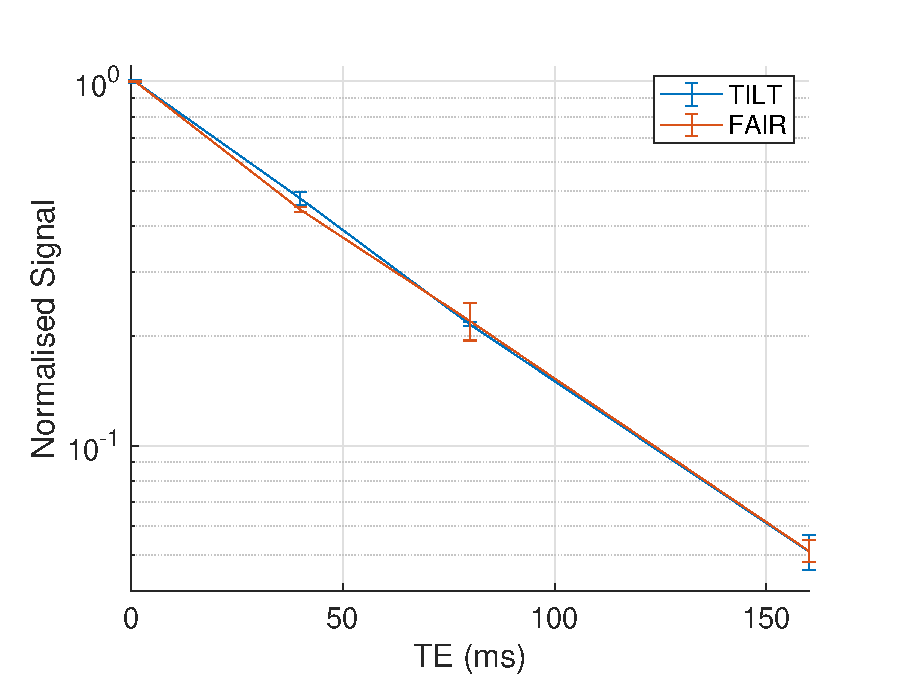
\includegraphics[width=0.55\textwidth]{TRUST/T2_brain_tilt_vs_fair_5.eps}
	\caption{The signal decay within the superior sagittal sinus measured using \ac{TRUST} for the \ac{TILT} and \ac{FAIR} labelling schemes scaled by their initial signal intensities at eTE = 1 ms.}
	\label{fig:TILT_vs_FAIR}	
\end{figure}

As can be seen these signals are in excellent agreement with the \ac{TILT} sequence yielding a venous blood \ttwo of $52\pm1$ ms corresponding to a $Y_v$ of $55\pm1~\%$ and the \ac{FAIR} sequence yielding a venous blood \ttwo of $50\pm2$ ms corresponding to a $Y_v$ of $53\pm2~\%$, therefore in agreement within the bounds of error. Having evaluated the accuracy of the \ac{FAIR} scheme to measure $Y_v$ in the superior sagittal sinus it was then be used for the renal \ac{TRUST} measurements.

First, the dependence of the signal on \ac{PLD} was measured with scans collected at a range of delays from 400 to 1400 ms for the \ac{FAIR} labelling scheme. The signal from \ac{eTE}=1 ms was then plot against label delay. Figure \ref{fig:Sig_vs_PLD_SS} shows the signal from the sagittal sinus from the brain \ac{FAIR} difference images. The maximum signal is observed with a \ac{PLD} of 800 ms. This value is reached due to the balance between \tone relaxation of the non-selective blood and inflow of unlabelled blood. This maximum in signal agrees with literature using the \ac{TILT} labelling scheme for assessing the sagittal sinus \cite{lu_quantitative_2008}. By carrying out scans with this \ac{PLD} the maximum \ac{SNR} will be achieved. 

\begin{figure}[H]
	\centering
	\includegraphics[width=0.55\textwidth]{TRUST/PLD_SS.eps}
	\caption{The mean signal from the first echo (\ac{eTE} = 1 ms) of each difference image over a range of \ac{PLD} times.}
	\label{fig:Sig_vs_PLD_SS}	
\end{figure}

\ttwo should have no dependence upon \ac{PLD} given the signal from the difference image will have the same decay in time, it will just be of lower intensity for a non-optimal \ac{PLD} thus leading to a larger confidence interval. To confirm this, the fit values of \ttwo in the sagittal sinus were plot against \ac{PLD}, Figure \ref{fig:SS_T2vsPLD}.

\begin{figure}[H]
	\centering
	\includegraphics[width=0.55\textwidth]{TRUST/T2_vs_PLD_SS.eps}
	\caption{The dependence of \ttwo in the sagittal sinus on \ac{PLD}.}
	\label{fig:SS_T2vsPLD}	
\end{figure}


It can be seen that, as predicted, there is no relationship between \ttwo and \ac{PLD}. An increase in error with label delay was not observed, this effect may only show itself at larger values of \ac{PLD} however here it is confirmed there is no large increase in error around the chosen \ac{PLD}. This means that if there is a variation in the optimum \ac{PLD} between subjects due to the larger range in \ac{RBF} compared to \ac{CBF} then this will not have an affect upon the value of \ttwo and thus $Y_v$.

To further evaluate the brain \ac{TRUST} data, an analysis was performed to assess the dependence of the measured \ttwo of blood in the sagittal sinus on number of voxels. Typically the four brightest voxels of the difference image are averaged before the fitting occurs, this number of voxels is chosen due to the average size of the superior sagittal sinus. The analysis was run multiple times with one to twelve voxels averaged before the calculation. Figure \ref{fig:nvox_SS} shows how \ttwo changes as the number of voxels included in the calculation is increased. %Multiple \ac{TRUST} scans were performed on the same subject and averaged generating Figure \ref{fig:nvox_SS}.

\begin{figure}[H]
	\centering
	\begin{subfigure}[c]{0.47\textwidth}
		\centering
		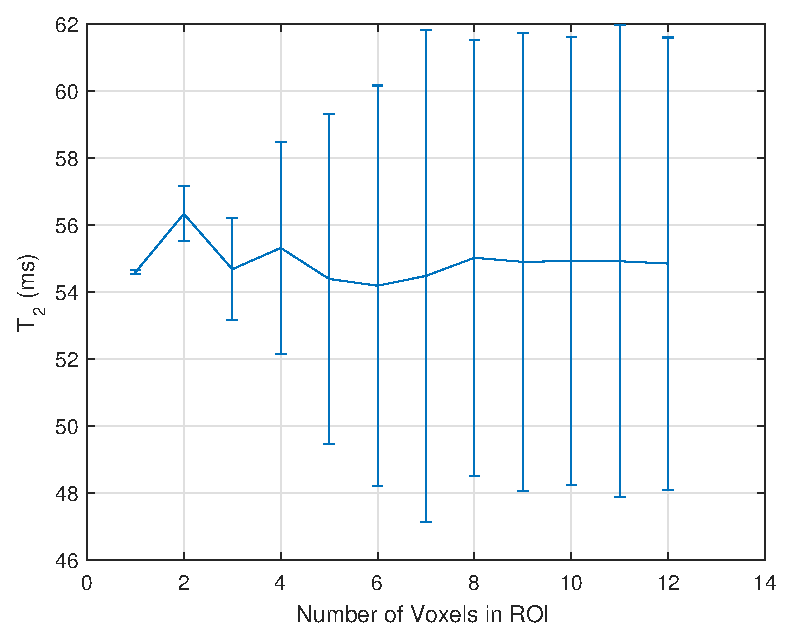
\includegraphics[width=0.9\textwidth]{TRUST/SS_T2_vs_nvox_mean2.eps}
		\caption{}
		\label{fig:nvox_SS}
	\end{subfigure}
	\hfill
	\begin{subfigure}[c]{0.47\textwidth}
		\centering
		\includegraphics[width=.7\textwidth, angle=270]{TRUST/SS_ROI}
		\caption{}
		\label{fig:SS_ROI}
	\end{subfigure}
	\caption{(\subref{fig:nvox_SS}) The value of \ttwo computed for the superior sagittal sinus as a function of the number of voxels included in the calculation. (\subref{fig:SS_ROI}) The difference image of the superior sagittal sinus with a three voxel \ac{ROI} shown. Note this size \ac{ROI} contains most of the sagittal sinus, hence the noise level drawn into the fit as more voxels are included in the calculation, as seen in (\subref{fig:nvox_SS}).}
	\label{fig:nv_SS}
\end{figure}

Although from Figure \ref{fig:nvox_SS} including only the brightest voxel yields a very small confidence interval and a similar \ttwo as the results with far more voxels; this would not be a very robust method. It is fairly easy to conceive a greater than average level of noise being recorded on a single voxel in the relaxation and as such skewing the output of the calculation. The confidence interval is so large above six voxels because by this point the calculations are simply including the noise around the vessel rather than the signal from the blood within the sagittal sinus. Given these results, using four voxels in the calculation produces a reasonable balance between uncertainty and robustness.

To assess the repeatability of this measure, the optimised scan was repeated ten times on a single subject during one scanning session. This yielded a $Y_v$ of $69.5\pm0.6$~\%, a value consistent with literature \cite{nagdyman_comparison_2005, liu_multi-site_2016}. Given the success of the modified sequence on the superior sagittal sinus, the respiratory triggered version of the sequence was then applied to attempt to measure $Y_v$ in the renal vein.

\subsubsection{\ac{TRUST} in the Body}

Ideal vessels to initially test the \ac{TRUST} sequence within the body are the portal vein and hepatic artery which feed the liver as these vessels are large and have very different oxygen saturations since the hepatic artery delivers oxygenated blood from the general circulation whilst the portal vein delivers deoxygenated blood from the small intestine. These vessels can easily be imaged at the same time in a single slice. Thus these vessels were evaluated using the modified \ac{TRUST} sequence. The \ttwo and oxygen saturation of the portal vein was found to be 109 $\pm$ 5 ms and 79.9 $\pm$ 0.8~\% respectively; the \ttwo and oxygen saturation of the hepatic artery was found to be 157 $\pm$ 10 ms and 100 $\pm$ 1~\% respectively. This shows that, as expected, the oxygen saturation in the hepatic artery is greater than that of the portal vein and therefore the \ac{TRUST} protocol it sensitive to the expected degrees of oxygenation in the body. Although normally the analysis would simply be based upon the mean of the brightest voxels in the difference image as outlined in Section \ref{sec:trust_analysis}, in Figure \ref{fig:pv_TRUST} a voxel-by-voxel analysis has been carried out for illustrative purposes. Note that far more voxels are available here than in the sagittal sinus

\begin{figure}[h]
	\centering
	\includegraphics[width=0.5\textwidth]{TRUST/PV_TRUSTmap.eps}
	\caption{The oxygen saturation of the portal vein and hepatic artery measured using \ac{TRUST} sequence.}
	\label{fig:pv_TRUST}	
\end{figure}
To assess if the \ac{PLD} that generates the greatest signal is the same in the renal vein as in the superior sagittal sinus, a series of \ac{TRUST} scans were collected with \ac{PLD} ranging from 400 ms to 1400 ms and the signal from \ac{eTE} = 1 ms plot.
%\begin{figure}[H]
%	\centering
%	\includegraphics[width=0.65\textwidth]{Signal_vs_Label_Delay_RV.eps}
%	\caption{The mean signal from the first echo of each difference image of the renal vein over a range of \ac{PLD}}
%	\label{fig:Sig_vs_PLD_RV}	
%\end{figure}

\begin{figure}[H]
	\centering
	\includegraphics[width=0.55\textwidth]{TRUST/PLD_RV.eps}
	\caption{The mean signal from the first echo (\ac{eTE} = 1 ms) of each difference image of the renal vein over a range of \acp{PLD}.}
	\label{fig:Sig_vs_PLD_RV}
\end{figure}

As seen in Figure \ref{fig:Sig_vs_PLD_RV} the \ac{PLD} producing the largest signal in the difference image of the renal vein is longer than that of the superior sagittal sinus. This is due to differences in labelling position and blood flow through each of these vessels, $413\pm136$ ml/min in the renal vein \cite{cox_multiparametric_2017} and $285\pm19$ ml/min in the superior sagittal sinus \cite{jordan_velocity_1994}. Given the much larger uncertainty in blood flow in the renal vein, an additional subject was scanned. The maximum signal for the first subject was achieved at a \ac{PLD} of 1200 ms whereas for the second subject the maximum is at a \ac{PLD} of 800 ms. Given there was little dependence of \ttwo upon \ac{PLD} at the peak, a \ac{PLD} of 1000 ms was chosen for optimum signal in most subjects.

Given the larger size of the renal vein compared to the superior sagittal sinus, it was assessed whether there would be an advantage in include more voxels in the calculations when fitting to compute of \ttwo. Three scans were acquired of the same subject, the value of \ttwo (and uncertainty in fit) was found using one to twelve voxels from each scan, \ttwo values of each scan were then averaged to generate Figure \ref{fig:nvox_RV}.  

\begin{figure}[H]
	\centering
	\begin{subfigure}[c]{0.47\textwidth}
		\centering
		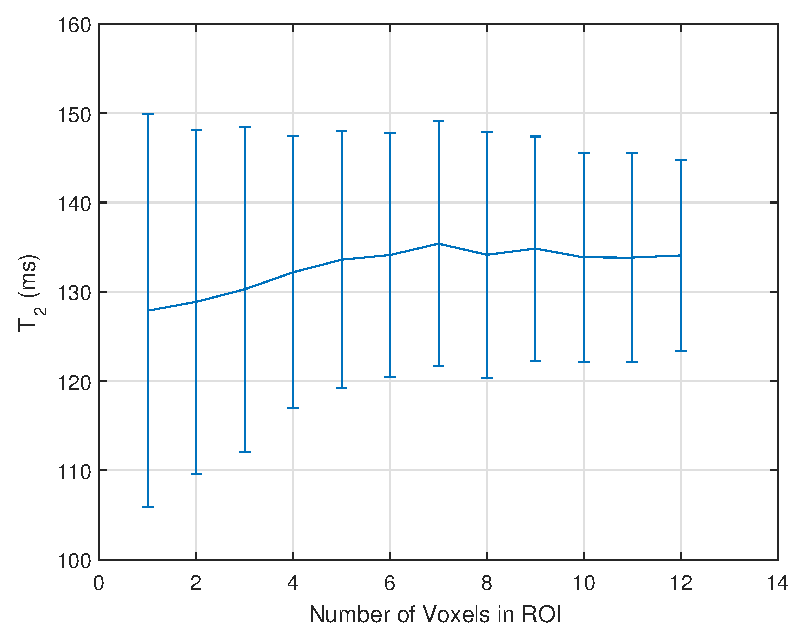
\includegraphics[width=1\textwidth]{TRUST/RV_T2_vs_nvox_mean_S2.eps}
		\caption{}
		\label{fig:nvox_RV}
	\end{subfigure}
	\hfill
	\begin{subfigure}[c]{0.47\textwidth}
		\centering
		\includegraphics[width=.7\textwidth]{TRUST/RV_ROI}
		\caption{}
		\label{fig:RV_ROI}
	\end{subfigure}
	\caption{(\subref{fig:nvox_RV}) The value of \ttwo calculated for the renal vein with different numbers of voxels included in the calculation. (\subref{fig:RV_ROI}) The difference image of the renal vein with a nine voxel \ac{ROI} shown.}
	\label{fig:nv_RV}
\end{figure}


Unlike the results for when this process was carried out on the superior sagittal sinus, Figure \ref{fig:nvox_SS}, here the error decreases as more voxels are added to the calculation. This uncertainty comes from the large variation in \ttwo for one voxel rather than a large error on the fit i.e. the error is coming from the differences between scans rather than the robustness of each scans results, this is precisely the concern that was raised with using a single voxel when discussing the superior sagittal sinus. As more voxels are added the error decreases until approximately six voxels are included, at this point the value of \ttwo plateaus to an approximate constant. Given the large variation in renal veins, this data suggests it would be advisable to include more voxels for the sagittal sinus. Nine voxels was chosen as a suitable middle ground as to work effectively with both small and large vessels.

To assess the repeatability of the measurements within the kidney, the same scan was repeated ten times in a single session with the optimised renal parameters, Figure \ref{fig:T2_Decay_Body}. This yielded a \ttwo of $135\pm5$ ms corresponding to a $Y_v$ of $89\pm2~\%$. The value of $Y_v$ in the renal vein is much higher than in the sagittal sinus however is within the range found by Nielsen \textit{et al} when drawing blood samples directly from the renal vein via insertion of a catheter and processing with an OSM$_2$ Radiometer to calculate $Y_v$ \cite{nielsen_renal_1992, saloojee_evaluation_1981}.

\begin{figure}[H]
	\centering
	\includegraphics[width=0.55\textwidth]{TRUST/T2_Decay_Body.eps}
	\caption{The \ttwo relaxation curves of ten scans repeated on a single subject.}
	\label{fig:T2_Decay_Body}	
\end{figure}

Finally, to compare the ability of \ac{BOLD} \ttwostar maps and \ac{TRUST} to measure changes in oxygenation in the kidneys, a hyperoxia challenge was conducted. In Figure \ref{fig:dT2star}, no systematic, bulk change in \ttwostar can be seen indicating that the change in \ttwostar caused by the introduction of pure oxygen is dominated by other confounding factors. This is confirmed when \ac{ROI} are defined for the renal cortex and renal medulla with the mean change in \ttwostar found to be $-2 \pm 8$ ms and $-1 \pm 6$ ms respectively. When \ac{TRUST} was used to measure the oxygen saturation in the renal vein an increase of 16 $\pm$ 3~\% was observed on hyperoxia, Figure \ref{fig:dYv}. This demonstrates that it is possible to measure changes in renal oxygenation using \ac{TRUST} that would be undetectable using the current standard, \ac{BOLD} \ttwostar mapping.
\begin{figure}[H]
	\centering
	\begin{subfigure}[c]{0.47\textwidth}
		\centering
		\includegraphics[width=1\textwidth]{TRUST/dT2star_M0.eps}
		\caption{}
		\label{fig:dT2star}
	\end{subfigure}
	\hfill
	\begin{subfigure}[c]{0.47\textwidth}
		\centering
		\includegraphics[width=1\textwidth]{TRUST/dYv_Sub_2.eps}
		\caption{}
		\label{fig:dYv}
	\end{subfigure}
	\caption{(\subref{fig:dT2star}), The difference in \ttwostar measured between baseline and the hyperoxia state. (\subref{fig:dYv}) The difference in $Y_v$ measured using \ac{TRUST}.}
	\label{fig:oxygen_chalenge_results}
\end{figure}

\newpage
\section{Conclusions and Future Work}

This work has demonstrated the implementation of a modified \ac{TRUST} sequence to measure oxygenation of blood within the body. The \ac{TRUST} sequence was modified for use in the abdomen by coding it to be respiratory triggered and use the \ac{FAIR} labelling scheme. Once these modifications had been carried out, parameters such as the \ac{PLD} and the number of voxels used in the \ac{ROI} were optimised. The sequence has been demonstrated initially on the portal vein and hepatic artery where the different degrees of deoxygenated and oxygenated blood can be mapped. The sequence is then developed for the assessment of renal vein oxygenation. The ability of \ac{TRUST} to measure a change in renal oxygenation was successfully verified via a hyperoxia challenge which was able to measure an increase of 16 $\pm$ 3~\% where the current standard measurement of renal oxygenation, \ac{BOLD} \ttwostar maps, recorded no significant change.

In future work this could be expanded by carrying out the hyperoxia challenge on more subjects. Although a small number of measurements were gathered on the hepatic vessels, further work could be undertaken to compare the use of \ac{SBO} and \ac{TRUST} to measure oxygenation in the portal vein in response to a hyperoxia challenge as conducted for the kidneys here. These methods could also be applied to the study of drugs on liver oxygenation. Due to limitations imposed by the \textsc{covid}-19 pandemic, performing further studies of hyperoxia has not been feasible. In the current protocol, the haematocrit is assumed to be an average value of 0.41 unless a blood test has recently been undertaken. As stated above, there is a correlation between \tone of blood and its haematocrit, this means that an estimate of the subjects haematocrit could be taken while they are in the scanner, thus leading to a more accurate measurement of oxygenation with only a small increase in scan time. This would be especially important when using \ac{TRUST} on patients rather than healthy volunteers as their haematocrit has a larger variance. By combining \ac{TRUST} measurements with \ac{PC}-\ac{MRI} measures, it is possible to estimate the \acf{RMRO$_2$}.

During the course of this PhD, the effects of \textsc{covid}-19 on the lungs has been well documented, however the effects of this disease on other organs, including the kidneys, is less well known. Initial reports show a high incidence of \ac{AKI} in \textsc{covid}-19 \cite{selby_covid-19_2020, fisher_aki_2020, gabarre_acute_2020} with other retrospective studies showing that \textsc{covid}-19 is an independent risk factor for \ac{AKI} \cite{kolhe_acute_2020-1, adapa_covid-19_2020}. It is hypothesised that \textsc{covid}-19 induces a reduction in renal oxygenation leading to \ac{AKI}. TheW modified \ac{TRUST} sequence developed in this thesis, in addition to other quantitative renal \ac{MRI} protocols, is currently being used to study \textsc{covid}-19 subjects to better understand the link between \ac{AKI} and the ongoing pandemic. Data is being collected in both the acute phase of \textsc{covid}-19 whilst patients are on ventilators and at follow-up. It has been demonstrated that in healthy subjects the renal venous oxygenation is of the order of 86 $\pm$ 7~\% whereas in \textsc{covid}-19 oxygenation of blood in the renal vein is of the order of 59 $\pm$ 8~\%. It may be that this hypoxia is the cause of inflammation in the kidney.

\section{Acknowledgements}

I thank Professor Hanzhang Lu for sharing the TRUST methodology.

\newpage
\section{References}
\defbibheading{bibliography}[\refname]{}
\printbibliography